% Preview of the generated midway artifacts in a two-column article (stand-in for the course template).
% Build: cd report && latexmk -pdf preview.tex
\documentclass[twocolumn,10pt]{article}
\usepackage[margin=0.75in]{geometry}
\usepackage{booktabs,graphicx,xcolor}
\newcommand{\tbd}{\textcolor{gray}{--}}  % same macro the course main.tex defines

\begin{document}
\twocolumn[{\section*{Midway artifacts (preview)}
Generated by \texttt{make report}. All ``ours'' numbers come from runs in \texttt{runs/}; \tbd\ means not run yet.\vspace{1em}}]
\footnotesize

% generated by midway/tables.py from runs/aggregate.json (runs/norsnorb_full250_s42)
\begin{table*}[t]
\centering\footnotesize
\setlength{\tabcolsep}{4pt}
\caption{Replication of BrickGPT (Pun et al., Table~1). Cells are \emph{paper / ours}; ours is the mean over the $n$ prompts and seeds shown under each column. $\pm$ is half the width of a 95\% percentile bootstrap CI (10{,}000 resamples over prompts). Rates are over all $n$ prompts; stability, CLIP and DINO are over valid builds only. Stability: min.\ stab.\ $=1-$max stress, mean stab.\ $=1-$mean stress (raw). Upstream caps stress at 1, so raw equals clipped and an unstable build has min.\ stab.\ 0. GPU: Tesla T4. \tbd: not run yet; n/r: not reported in the paper.}
\label{tab:replication}
\begin{tabular}{lccc}
\toprule
 & No RS, no RB & RS only & RS + RB \\
\scriptsize ours: & \scriptsize full250, n=250, s42 & \scriptsize \tbd & \scriptsize \tbd \\
\midrule
\% valid & 37.2 / 36.4\textsubscript{\,$\pm$6.0} & 100.0 / \tbd & 100.0 / \tbd \\
\% stable & 12.8 / 12.8\textsubscript{\,$\pm$4.2} & 24.0 / \tbd & 98.8 / \tbd \\
Mean stab. & 0.956 / 0.960\textsubscript{\,$\pm$0.01} & 0.947 / \tbd & 0.996 / \tbd \\
Min.\ stab. & 0.325 / 0.322\textsubscript{\,$\pm$0.09} & 0.228 / \tbd & 0.915 / \tbd \\
CLIP & 0.329 / \tbd & 0.322 / \tbd & 0.324 / \tbd \\
DINO & 0.888 / \tbd & 0.882 / \tbd & 0.880 / \tbd \\
Rollbacks (median) & n/a (RB off) & n/a (RB off) & 2.0 / \tbd \\
Sec.\ per build (median) & n/r / 26.0\textsubscript{\,$\pm$2.8} & n/r / \tbd & 40.8 / \tbd \\
\bottomrule
\end{tabular}
\end{table*}

% generated by midway/tables.py from runs/aggregate.json (runs/rs_full250_s42, runs/full_first30_s42)
\begin{table*}[t]
\centering\footnotesize
\setlength{\tabcolsep}{4pt}
\caption{Main comparison (RQ2/RQ3). Stable@1: \% stable with rejection sampling and no rollback. Final \% stable, rollbacks (median), sec./build (median): full decoding with rollback. IoU: voxel IoU with the ground-truth build. BrickGPT Stable@1 is from the RS-only run (full250, n=250, s42); its other columns are from the RS+RB run (first30, n=24 of 30, s42). $\pm$ is half the width of a 95\% percentile bootstrap CI (10{,}000 resamples over prompts). \tbd: not run yet.}
\label{tab:main}
\begin{tabular}{lcccccccc}
\toprule
Model & Stable@1 & Final \% stable & Rollbacks & Sec./build & CLIP & DINO & IoU & \#bricks \\
\midrule
BrickGPT (ours) & 23.2\textsubscript{\,$\pm$5.0} & 95.8\textsubscript{\,$\pm$6.2} & 3.0\textsubscript{\,$\pm$1.5} & 137.1\textsubscript{\,$\pm$90.7} & \tbd & \tbd & 0.251\textsubscript{\,$\pm$0.08} & 79.5\textsubscript{\,$\pm$15.1} \\
RFT & \tbd & \tbd & \tbd & \tbd & \tbd & \tbd & \tbd & \tbd \\
DPO-seq & \tbd & \tbd & \tbd & \tbd & \tbd & \tbd & \tbd & \tbd \\
DPO-prefix (BrickDPO) & \tbd & \tbd & \tbd & \tbd & \tbd & \tbd & \tbd & \tbd \\
DPO-local (ours) & \tbd & \tbd & \tbd & \tbd & \tbd & \tbd & \tbd & \tbd \\
\bottomrule
\end{tabular}
\end{table*}

% generated by midway/tables.py from runs/aggregate.json (no runs yet)
\begin{table}[t]
\centering\footnotesize
\setlength{\tabcolsep}{4pt}
\caption{Window-size sweep for DPO-local at a fixed pair budget (RQ3). \tbd: not run yet.}
\label{tab:window}
\begin{tabular}{lcccc}
\toprule
Model & Stable@1 & Rollbacks & \#bricks & IoU \\
\midrule
DPO-local, $m=1$ & \tbd & \tbd & \tbd & \tbd \\
DPO-local, $m=5$ & \tbd & \tbd & \tbd & \tbd \\
DPO-local, $m=20$ & \tbd & \tbd & \tbd & \tbd \\
\bottomrule
\end{tabular}
\end{table}

% generated by midway/tables.py from runs/aggregate.json (no runs yet)
\begin{table*}[t]
\centering\footnotesize
\setlength{\tabcolsep}{4pt}
\caption{Shape-filter ablation (RQ4). Height: layers; footprint: occupied cells seen from above; \% 1$\times$1: share of 1$\times$1 bricks; shape statistics are over all parsed builds. BrickGPT Stable@1 from the RS-only run (\tbd), other columns from the RS+RB run (\tbd). $\pm$ is half the width of a 95\% percentile bootstrap CI (10{,}000 resamples over prompts). \tbd: not run yet.}
\label{tab:shape}
\begin{tabular}{lcccccccc}
\toprule
Model & Stable@1 & CLIP & DINO & IoU & \#bricks & Height & Footprint & \% 1$\times$1 \\
\midrule
DPO-local, with IoU filter & \tbd & \tbd & \tbd & \tbd & \tbd & \tbd & \tbd & \tbd \\
DPO-local, no IoU filter & \tbd & \tbd & \tbd & \tbd & \tbd & \tbd & \tbd & \tbd \\
BrickGPT (reference) & \tbd & \tbd & \tbd & \tbd & \tbd & \tbd & \tbd & \tbd \\
\bottomrule
\end{tabular}
\end{table*}


\begin{figure}[t]
  \centering
  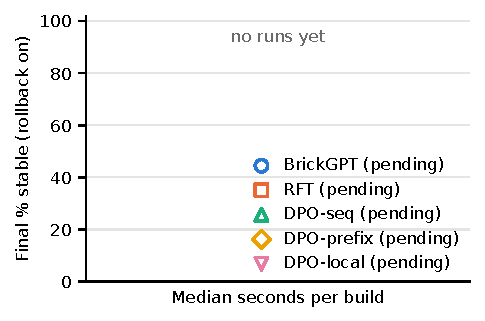
\includegraphics[width=\columnwidth]{figures/fig2_stability_vs_cost}
  \caption{Stability vs.\ cost (RQ5): median seconds per build vs.\ final \% stable with rollback, 95\% bootstrap
  CIs. Hollow legend markers are models not yet run.}
  \label{fig:cost}
\end{figure}

\begin{figure}[t]
  \centering
  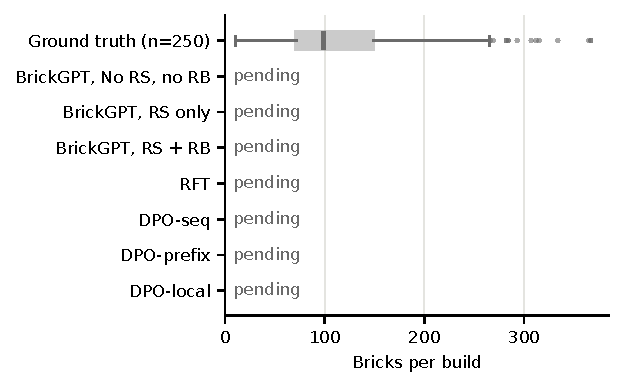
\includegraphics[width=\columnwidth]{figures/fig3_brick_counts}
  \caption{Bricks per build. Box: quartiles; line: median; whiskers: 1.5 IQR. A shift right relative to
  BrickGPT would indicate build inflation.}
  \label{fig:bricks}
\end{figure}

\begin{figure}[t]
  \centering
  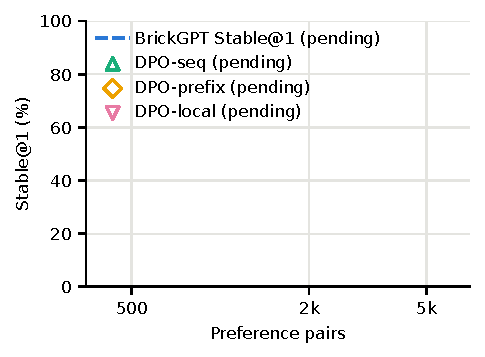
\includegraphics[width=\columnwidth]{figures/fig4_stable_vs_pairs}
  \caption{Stable@1 vs.\ preference-pair budget (RQ3). Dashed line and band: BrickGPT Stable@1 and its 95\% CI.}
  \label{fig:pairs}
\end{figure}

\end{document}
